\chapter{Auxiliary Plots for Symbolic Error-propagation Experiments on \textsc{LTLZinc-Sequential}}\label{app:ltlzincoracle}
Figures \ref{ijcai:fig:abl-avg}, \ref{ijcai:fig:abl-const} and \ref{ijcai:fig:abl-succ} show the behavior of symbolic methods fed with oracular predictors (Error-propagation experiments), for every task. For readability, Figure~\ref{ijcai:fig:abl-task4-nolimits} shows accuracies for Task 4 side by side (this is the uncropped  version of Figure~\ref{ijcai:fig:abl-task4} in the main text).

\begin{figure*}
	\centering
	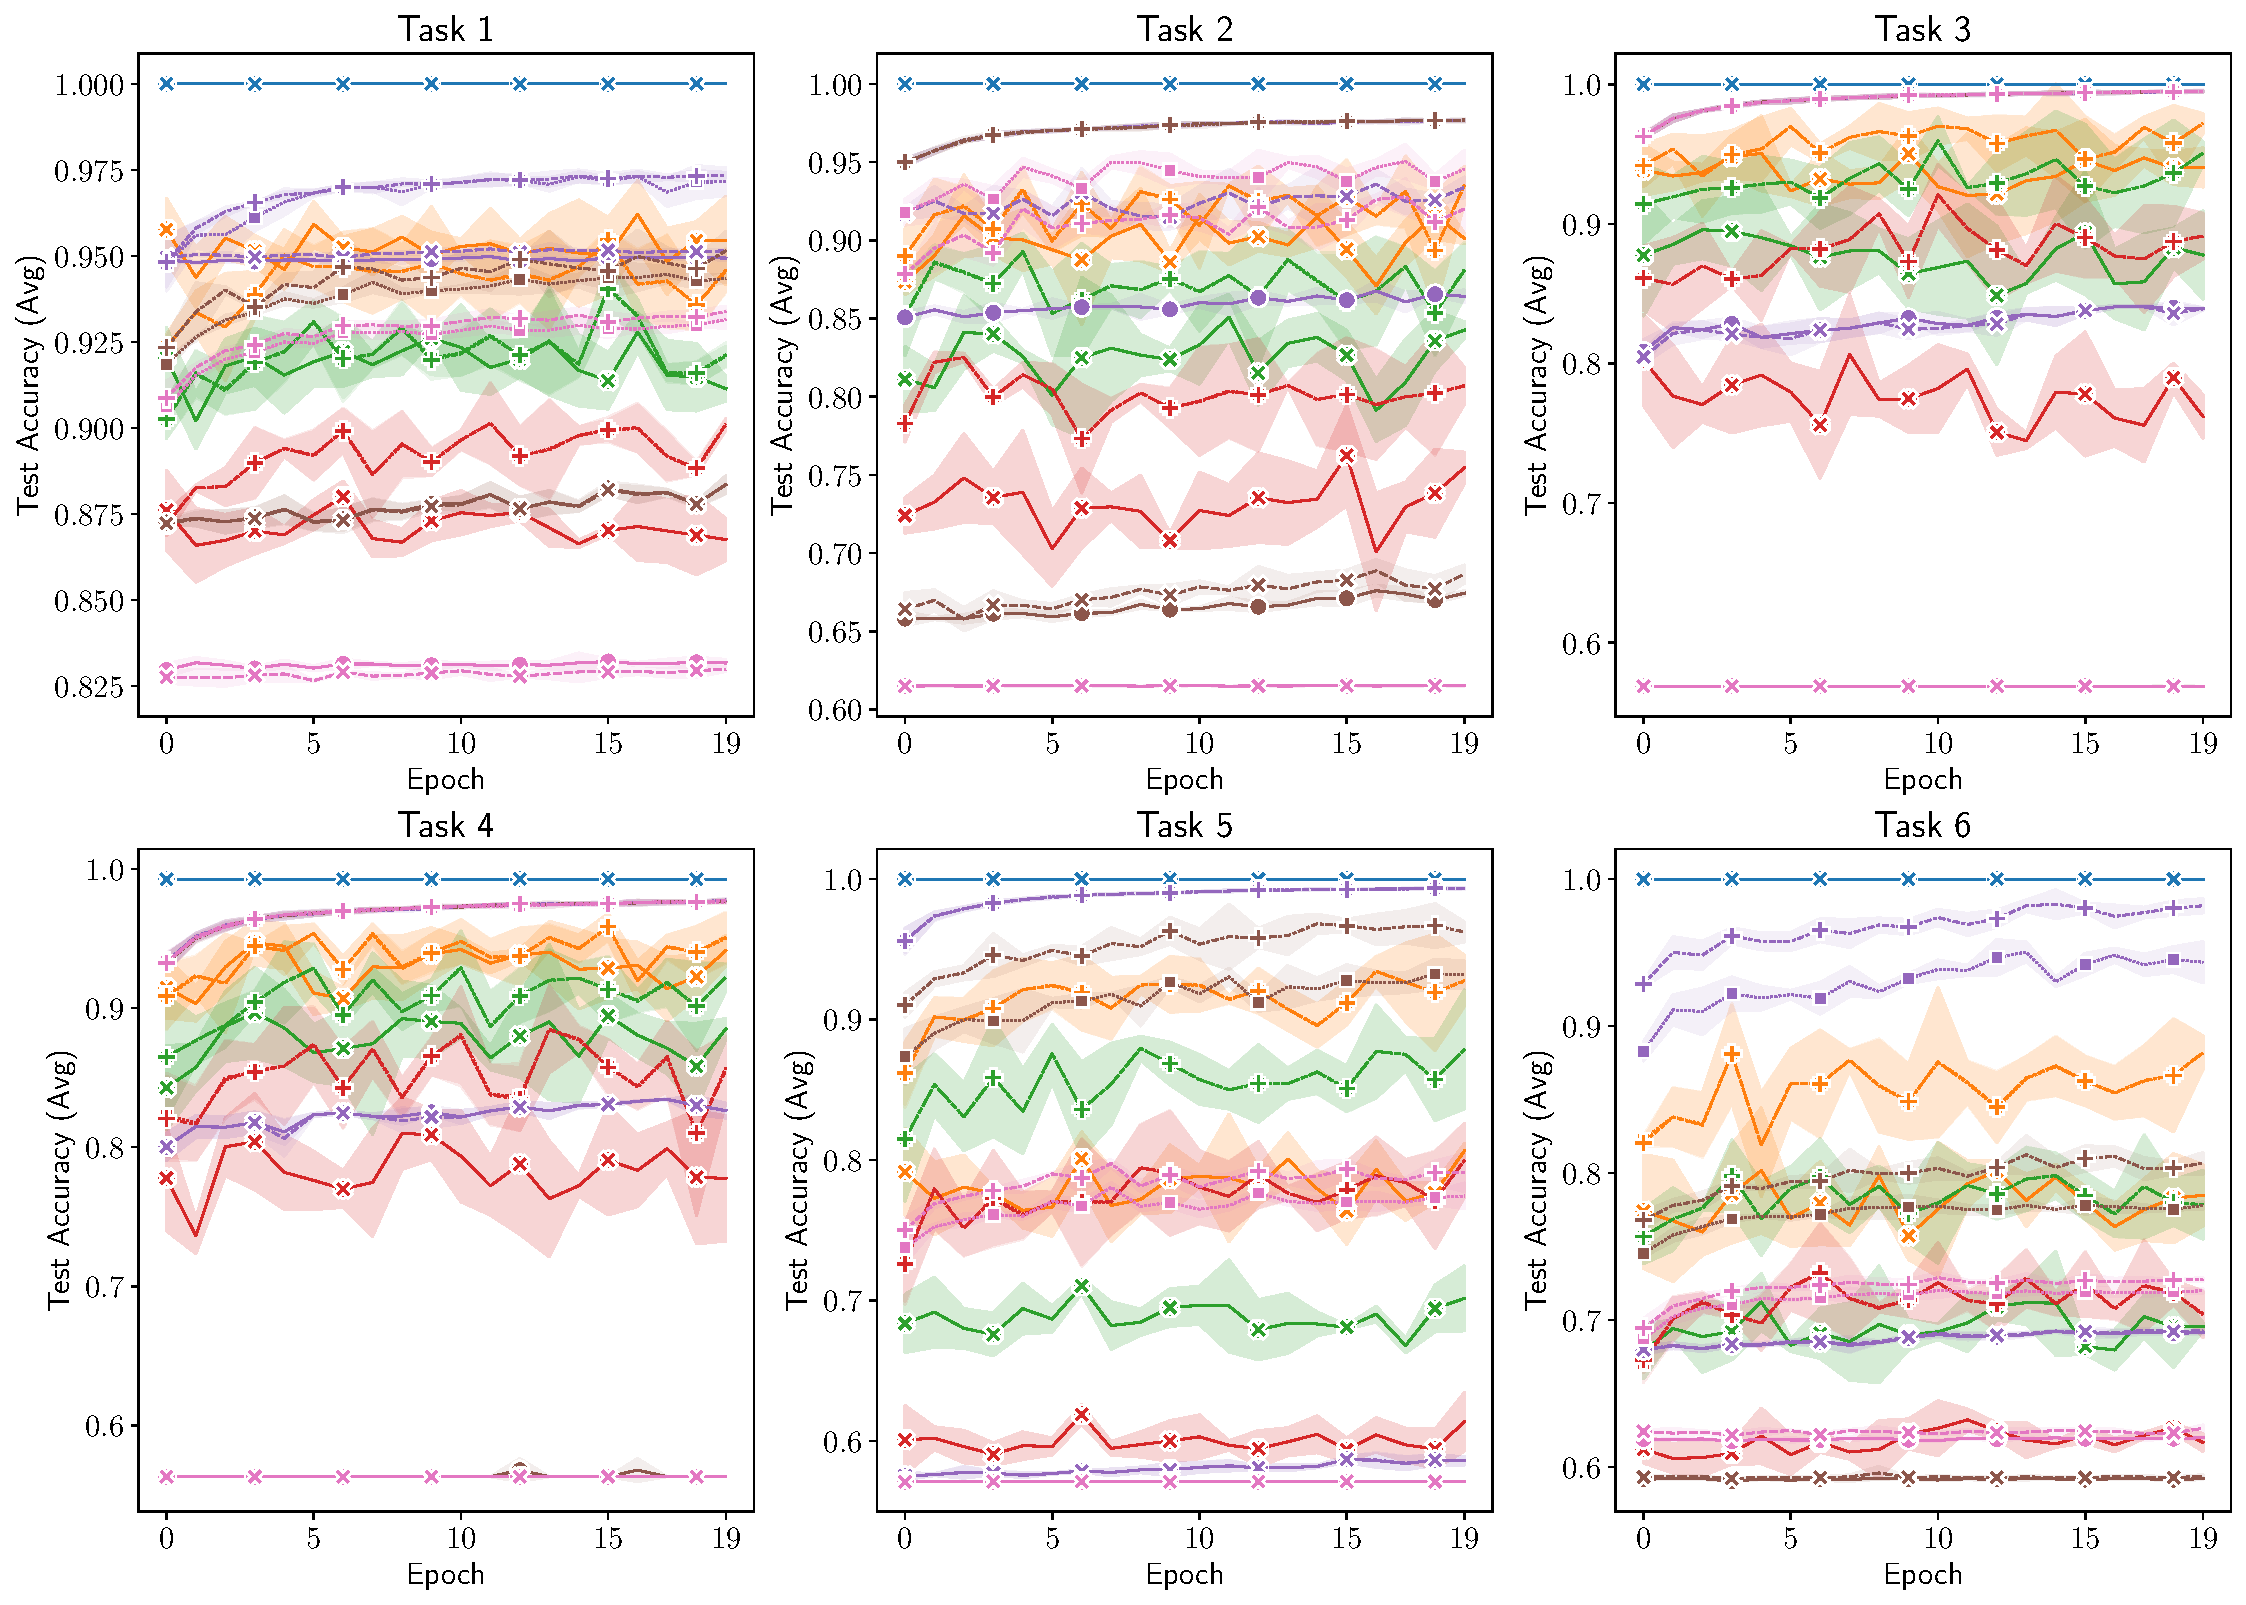
\includegraphics[width=\linewidth]{imgs/ijcai/ablation_avg_full.pdf}
	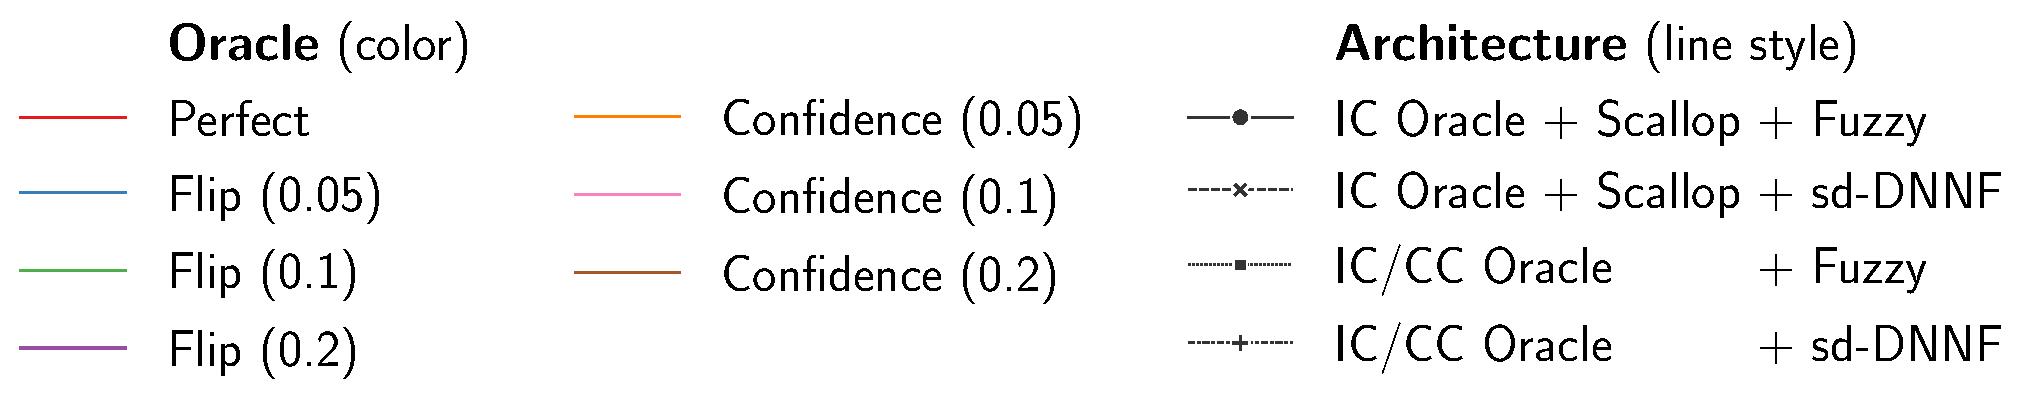
\includegraphics[width=\linewidth]{imgs/ijcai/ablation_task4_legend.pdf}
	\caption{Average accuracy when replacing \textsc{IC} or \textsc{IC/CC} modules with an oracular predictor.}
	\label{ijcai:fig:abl-avg}
\end{figure*}

\begin{figure*}
	\centering
	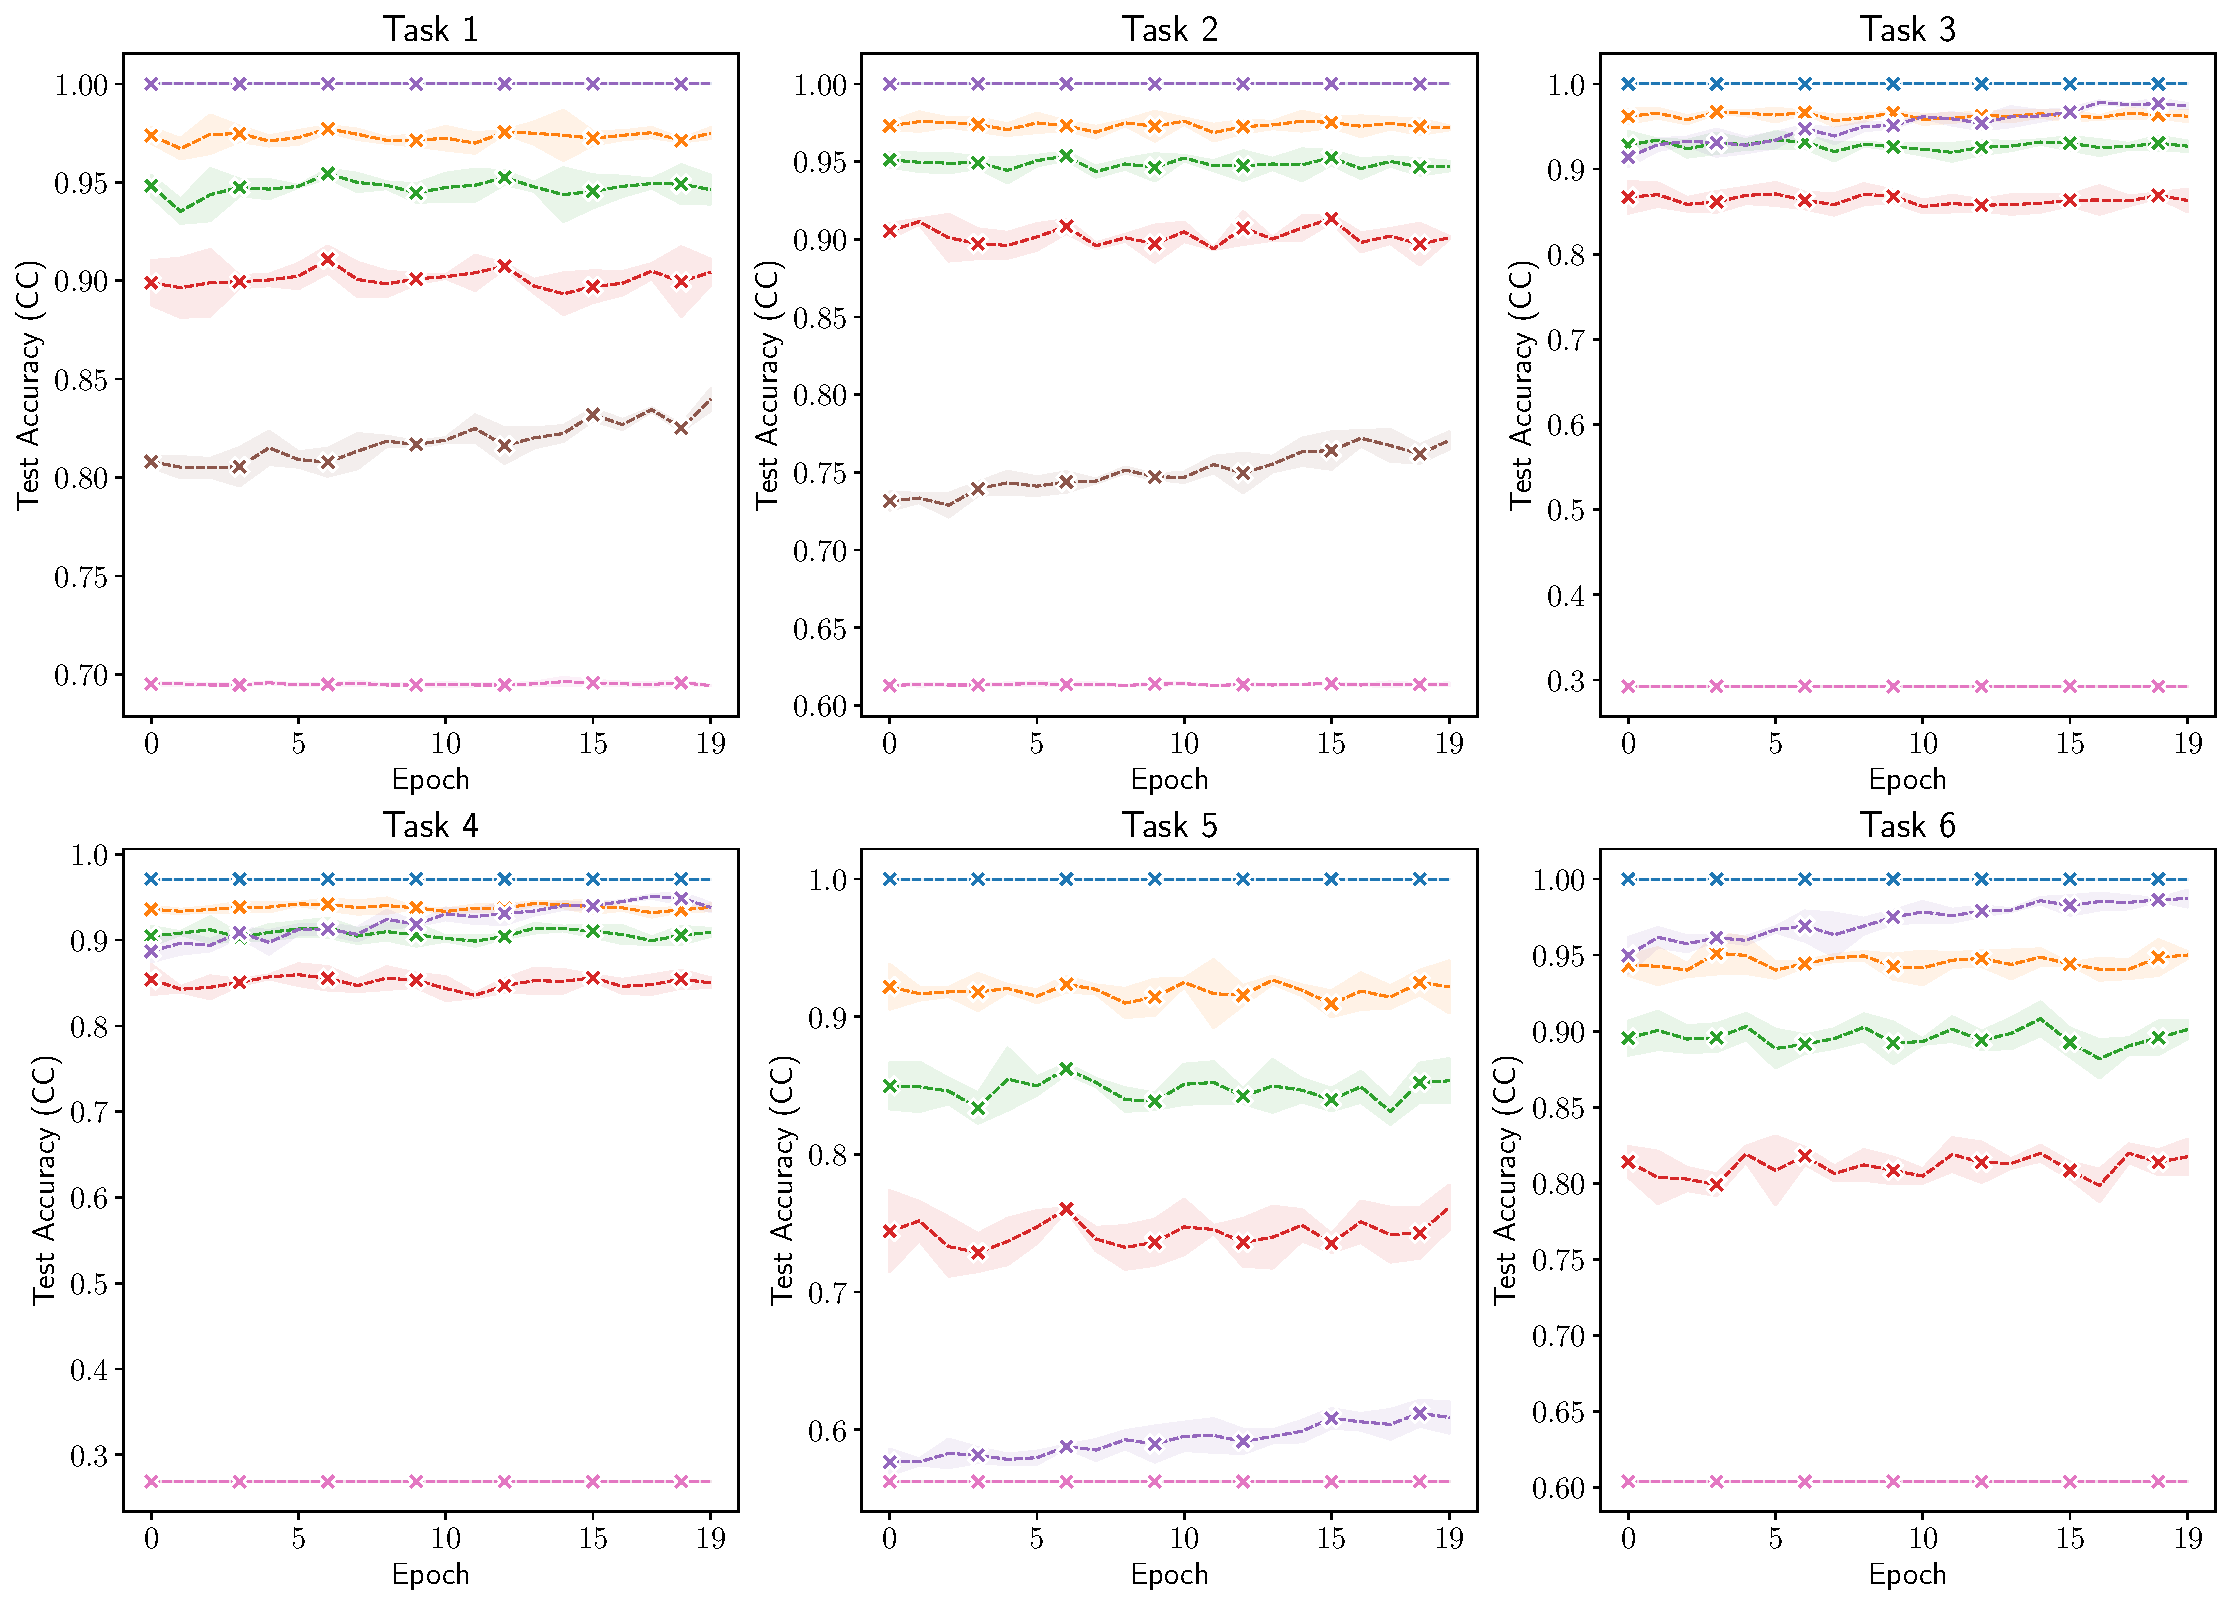
\includegraphics[width=\linewidth]{imgs/ijcai/ablation_constraint_full.pdf}
	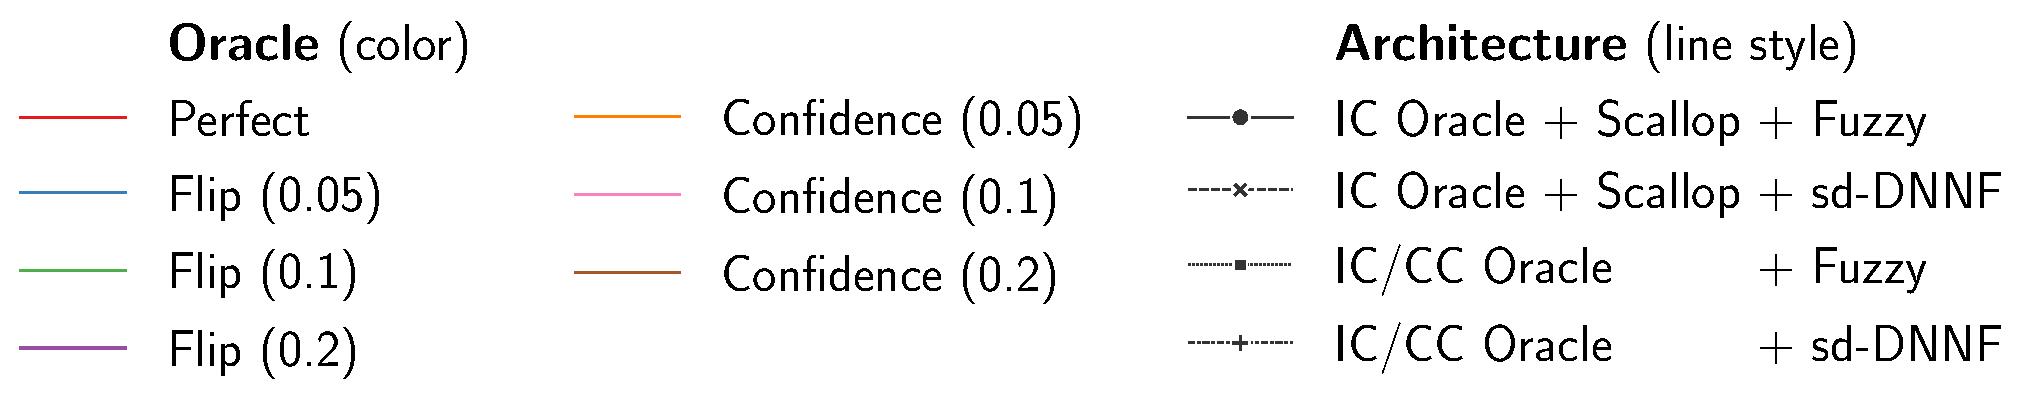
\includegraphics[width=\linewidth]{imgs/ijcai/ablation_task4_legend.pdf}
	\caption{\textsc{CC} accuracy when replacing \textsc{IC} or \textsc{IC/CC} modules with an oracular predictor. For readability, \textsc{IC/CC} results are suppressed (they trivially achieve $1.0$ \textsc{CC} accuracy, as the argmax is the same as the perfect oracle). Only one \textsc{NSP} module is shown, as they do not affect \textsc{CC} performance.}
	\label{ijcai:fig:abl-const}
\end{figure*}

\begin{figure*}
	\centering
	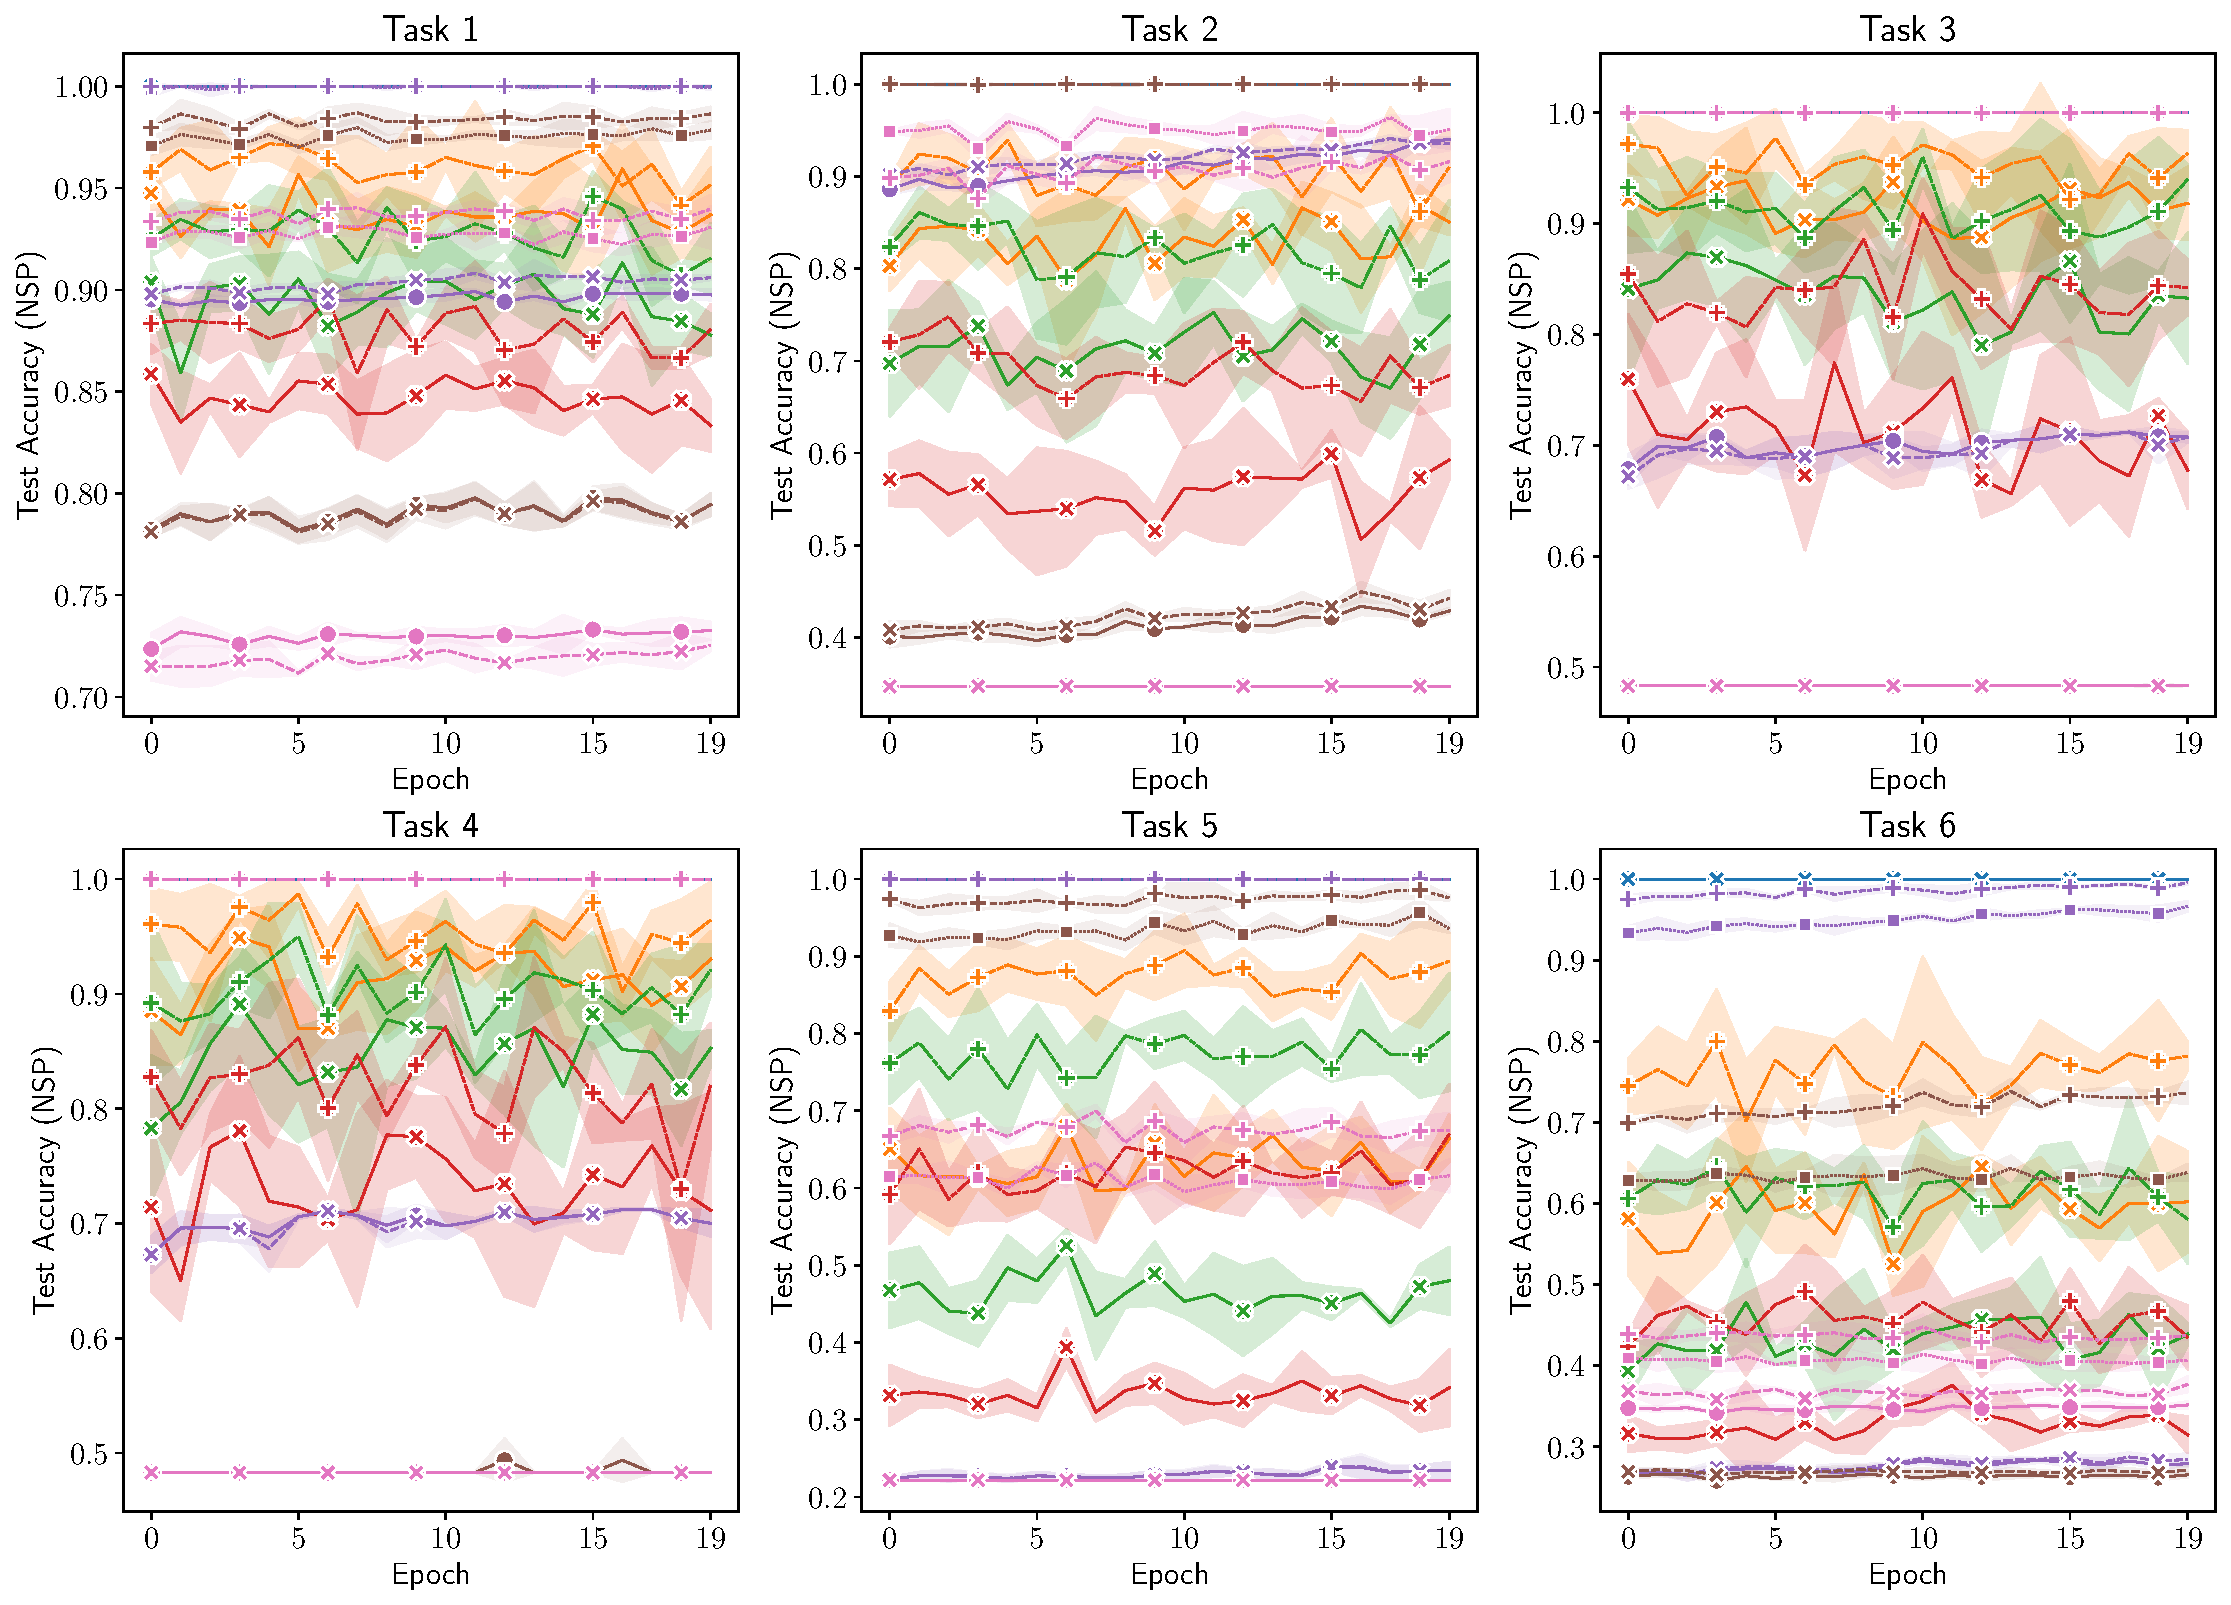
\includegraphics[width=\linewidth]{imgs/ijcai/ablation_successor_full.pdf}
	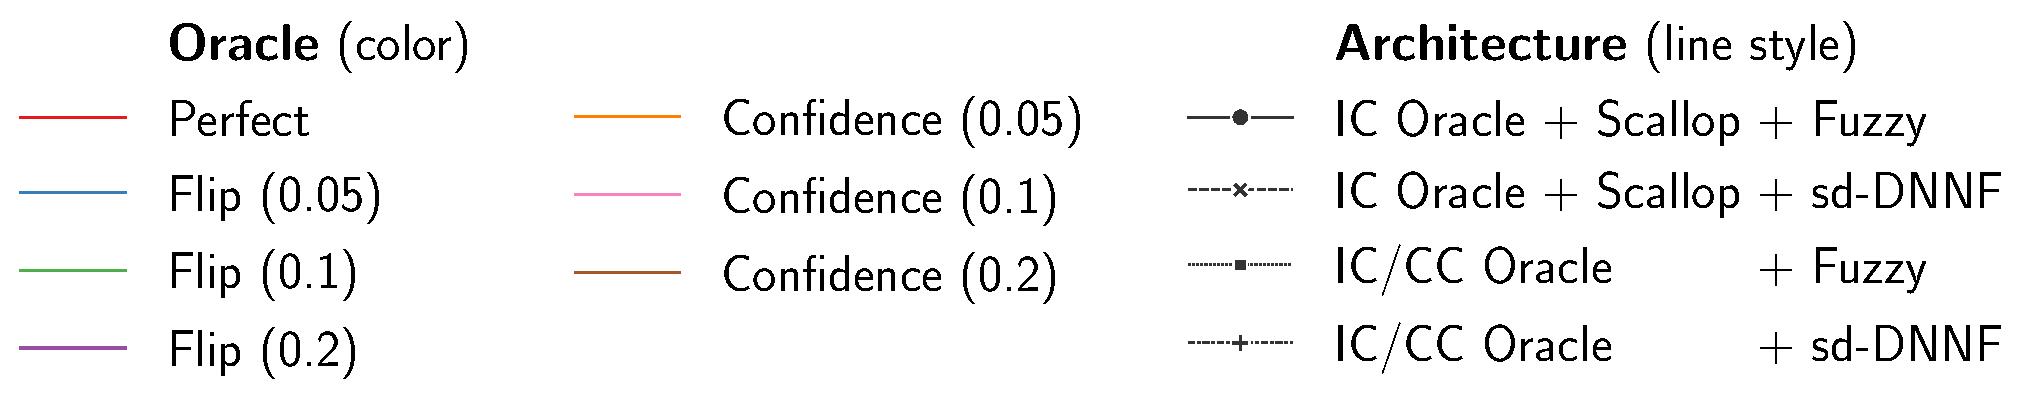
\includegraphics[width=\linewidth]{imgs/ijcai/ablation_task4_legend.pdf}
	\caption{\textsc{NSP} accuracy when replacing \textsc{IC} or \textsc{IC/CC} modules with an oracular predictor.}
	\label{ijcai:fig:abl-succ}
\end{figure*}

\begin{figure*}
	\centering
	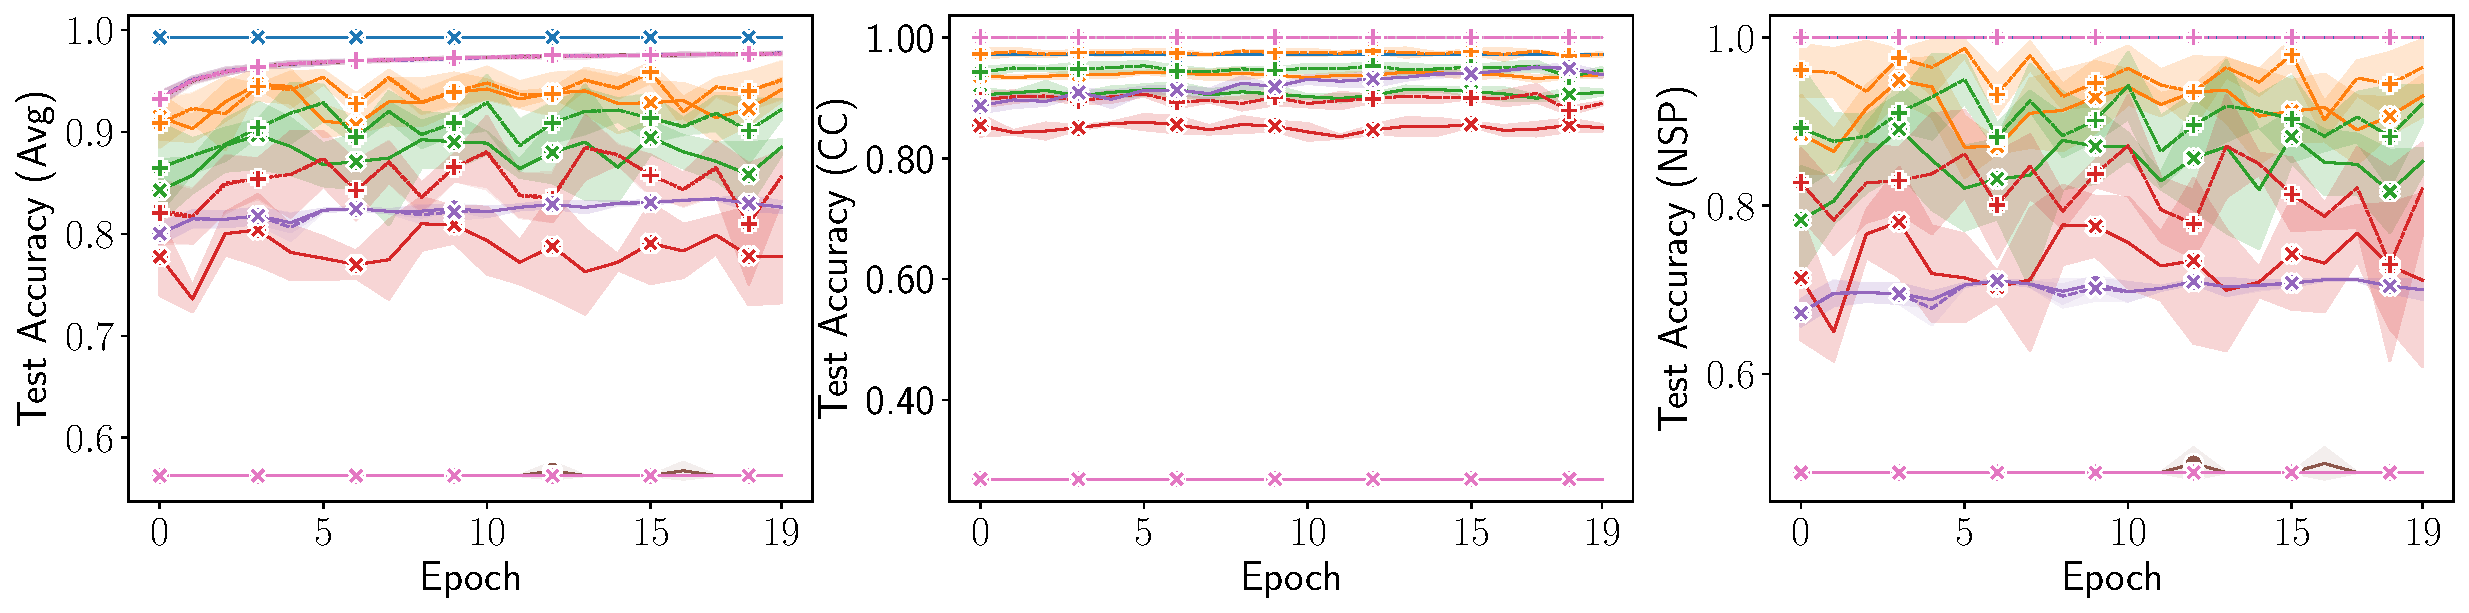
\includegraphics[width=\linewidth]{imgs/ijcai/ablation_task4_full.pdf}
	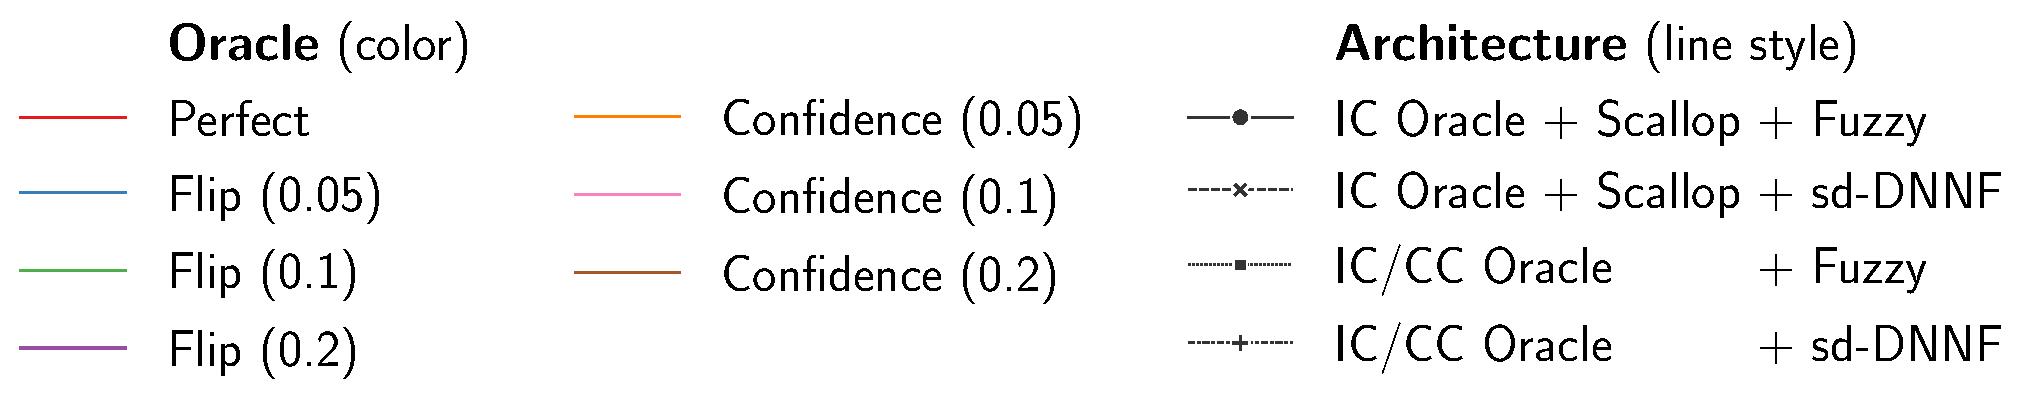
\includegraphics[width=\linewidth]{imgs/ijcai/ablation_task4_legend.pdf}
	\caption{Accuracies for \textit{Task 4} with oracular predictors. These are the same data points as Figure~\ref{ijcai:fig:abl-task4} in the main text, showing also curves below threshold accuracy.}
	\label{ijcai:fig:abl-task4-nolimits}
\end{figure*}